\chapter{Diseño de la experimentación}\label{cap:disegno_experimento}
%DESCOMENTAR ESTAS LÍNEAS SI EL CAPÍTULO TIENE FIGURAS O TABLAS
\addtocontents{lof}{{\bf \noindent Figuras del capítulo \arabic{chapter}}}
\addtocontents{lot}{{\bf \noindent Tablas del capítulo \arabic{chapter}}}

\section{Lógica del diseño}\label{cap:logica_diseno}
\section{Estructuras de datos de los problemas}
\paragraph{Algoritmo de Prim}
\paragraph{Algoritmo de Dijkstra}
\paragraph{PACMG}
\paragraph{PCMG}
\paragraph{PVVG}

\section{Identificación de Componenetes Elementales}\label{cap:identificacion_componentes}


\subsection{Descomponiendo Algoritmo Dijkstra}
El algoritmo de Dijkstra permite resolver de forma polinomial el problema del camino mínimo
y en el algoritmo 5.1 se presenta su pseudocódigo.

\begin{algorithm}[H]
    \begin{algorithmic}[1]
        \STATE {\em Inicializar Etiquetas con antecesor nulo y costo INFINITO}
        \STATE {\em Inicializar una lista L con Todos los vétices del Grafo}
        \STATE {\em Etiquetar Vértice Inicial=[-,0]}
        \STATE {\em Marcar X = vértice Inicial}
        \STATE {\em Eliminar Vértice Incial de L}
        \WHILE {{\em Quedan Vértices en lista L}}
            \STATE {\em Actualizar etiquetas vecinos de X solo si el costo es menor.}
            \STATE {\em Buscar en L, el nodo con Etiqueta con costo más bajo (Nmin).}
            \STATE {\em Macar X=Nmin.}
            \STATE {\em Eliminar Nmin de L}
        \ENDWHILE
    \end{algorithmic}
    \caption{Algoritmo de Dijkstra}\label{alg:alg41}
\end{algorithm}

En las lineas 1 hasta la 5 permiten inicializar las estructuras, mientras que en la línea 6 se puede observar el ciclo que permite realizar las iteraciones hasta encontrar el camino mínimo. La línea 7 es la encargada de actualizar las etiquetas de los vecinos del vértice seleccionado; la línea 8 busca en la lista de nodos disponibles el vértice seleccionado; la línea 9 es la encargada de marcar el vértice en la solución. Finalmente la línea 10 es la que elimina el vértice marcado de la lista de vértices disponibles.

De esta forma el algoritmo se ejecuta hasta que todos los vértices hayan sido marcados. Esto se cumple con el criterio de término del ciclo \emph{while} del pseudocódigo, ya que a medida que se extraen los nodos de la lista \emph{L}, se van marcando y etiquetando los vértices del grafo.

Se puede observar que los componentes elementales del algoritmo están en la línea 6, que es la que permite que el ciclo siga hasta encontrar la solución, línea 7, encargada de actualizar las etiquetas y la línea 9  marcar el vértice en la solución. Generando así los siguientes terminales:




\subsection{Descomponiendo Algoritmo Prim}
\begin{algorithm}[H]
    \caption{Algoritmo de Dijkstra}\label{alg:alg41}
    \begin{algorithmic}[1]
        \STATE Inicializar el árbol con un vértice arbitrario.
        \WHILE {{\em Quedan Vértices sin utilizar}}
            \STATE Añadir la arista de menor peso que se conecte con el árbol.
        \ENDWHILE
    \end{algorithmic}
\end{algorithm}

\section{Diseño de componentes elementales}
\section{Instancias}
\section{Lógica del diseño}\label{cap:logica_diseno}

\section{Experimentos PG tradicional}\label{cap:experimento_tradicional}
Para el desarrollo de este experimento se utiliza la PG tradicional que fue descrita en \ref{cap:pg}. Este experimento está dividido en dos etapas: proceso evolutivo o de evolución y el proceso de evaluación.

\subsection{El proceso evolutivo}
Se considera un proceso de aprendizaje donde se identifica la combinación adecuada de elementos que permitan resolver el problema. Para lograrlo es necesario realizar los siguientes pasos:

\begin{itemize}
  \item Definir una estructura de datos.
  \item Definir un conjunto de funciones y terminales, que cumplan con las propiedades de suficiencia y clausura.
  \item Construir una función de evaluación acorde al problema para evaluar el rendimiento de los algoritmos generados.
  \item Seleccionar un conjunto de instancias del problema para adaptar los algoritmos a generar (grupo de instancias de evolución).
  \item Determinar los métodos evolutivos y el valor de los parámetros de control del proceso evolutivo.
  \item Ejecutar el proceso evolutivo un número determinado de veces y recopilar estadísticas de los individuos generados.
  \item Seleccionar un conjunto de individuos para ser estudiados.
\end{itemize}

\subsection{El proceso de evaluación}
En este proceso se mide el desempeño computacional que tienen los algoritmos producidos en el proceso evolutivo. Consiste en medir la calidad de los algoritmos generados. La calidad de los algoritmos se determina a partir de que tan bien resuelve el problema y cuánto tiempo tarda en hacerlo. Para ello, se selecciona un conjunto de instancias distinto al grupo de instancias de evolución y los algoritmos son evaluados en este nuevo conjunto. Para medir la calidad de los algoritmos evaluados en el conjunto de evaluación, se utiliza el ERP (error relativo promedio), que consiste en el error relativo de los algoritmos obtenidos. Para cada grupo de instancias de evaluación $S$, se determina el porcentaje promedio por el cual el beneficio obtenido $z_{i}$ se encuentra distanciado de la mejor solución $o_{i}$ para cada instancia del conjunto $S$. Esto se representa en la ecuación \ref{eq:ERP_cap3}, donde $n_{s}$ representa el número de instancias del conjunto $S$.

\begin{equation}
  \label{eq:ERP_cap3}
  ERP_{s} =  \frac{1}{n_{s}} \cdot \sum\limits_{i=1}^{n_{s}} \frac{z_{i} - o_{i}}{z_{i}} \cdot 100\%
\end{equation}

\section{Experimentos PG con co-evolución mediante uso de islas}\label{cap:experimento_islas}
Para el desarrollo de este experimento se utiliza el método de co-evolución mediante el uso de islas basado en el principio de que los requisitos estrictos representados con una función de evaluación, promueven mejores resultados de la evolución de la primera población \citep{shang_2014}. Este experimento también se encuentra dividido en dos etapas: el proceso evolutivo o evolución y el proceso de evaluación.

\subsection{El proceso evolutivo}
Al igual que en el caso tradicional, se considera un proceso de aprendizaje, donde se identifica la combinación adecuada de elementos que permitan resolver el problema. Sin embargo, los pasos para desarrollar este proceso difieren en algunos puntos. Los pasos para este experimento son:

\begin{itemize}
  \item Definir una estructura de datos.
  \item Definir un conjunto de funciones y terminales, que cumplan con las propiedades de suficiencia y clausura.
  \item Construir dos funciones de evaluación acorde al problema para evaluar el rendimiento de los algoritmos generados.
  \item Seleccionar dos conjuntos de instancias del problema para adaptar los algoritmos a generar (grupo de instancias de evolución).
  \item Determinar los métodos evolutivos y el valor de los parámetros de control del proceso evolutivo.
  \item Determinar el número de individuos a intercambiar entre cada una de las islas, cada cuántas generaciones se realiza este cambio y entre qué islas se realiza el cambio.
  \item Ejecutar el proceso evolutivo un número determinado de veces y recopilar estadísticas de los individuos generados.
  \item Seleccionar un conjunto de individuos para ser estudiados.
\end{itemize}

En el experimento de co-evolución utilizando el método de islas para la PG, cada una de las islas opera usando la PG de forma tradicional. La interacción que se produce en estas islas es cada un determinado número de generaciones. En esta interacción se envía una copia de un grupo de los mejores individuos de cada isla a las demás y, a su vez, cada una de las islas elimina sus peores individuos para tener la “capacidad” o “espacio” para recibir a los inmigrantes manteniendo el tamaño de la población establecida.

El experimento se encuentra representando en las imágenes de la Figura \ref{fig:simbologia} a la Figura \ref{fig:final_islas}. En la Figura \ref{fig:simbologia} es posible apreciar la simbología a utilizar, donde se muestra que hay dos funciones de evaluación y dos conjuntos de instancias como se menciona en los pasos preparatorios descritos anteriormente. A continuación, en la Figura \ref{fig:estructura} es posible apreciar las cuatro islas formadas que conforman el experimento, donde en cada una de ella habitan individuos que se han adaptado mediante el proceso evolutivo de la PG tradicional.

\begin{figure}[H]
    \centering
    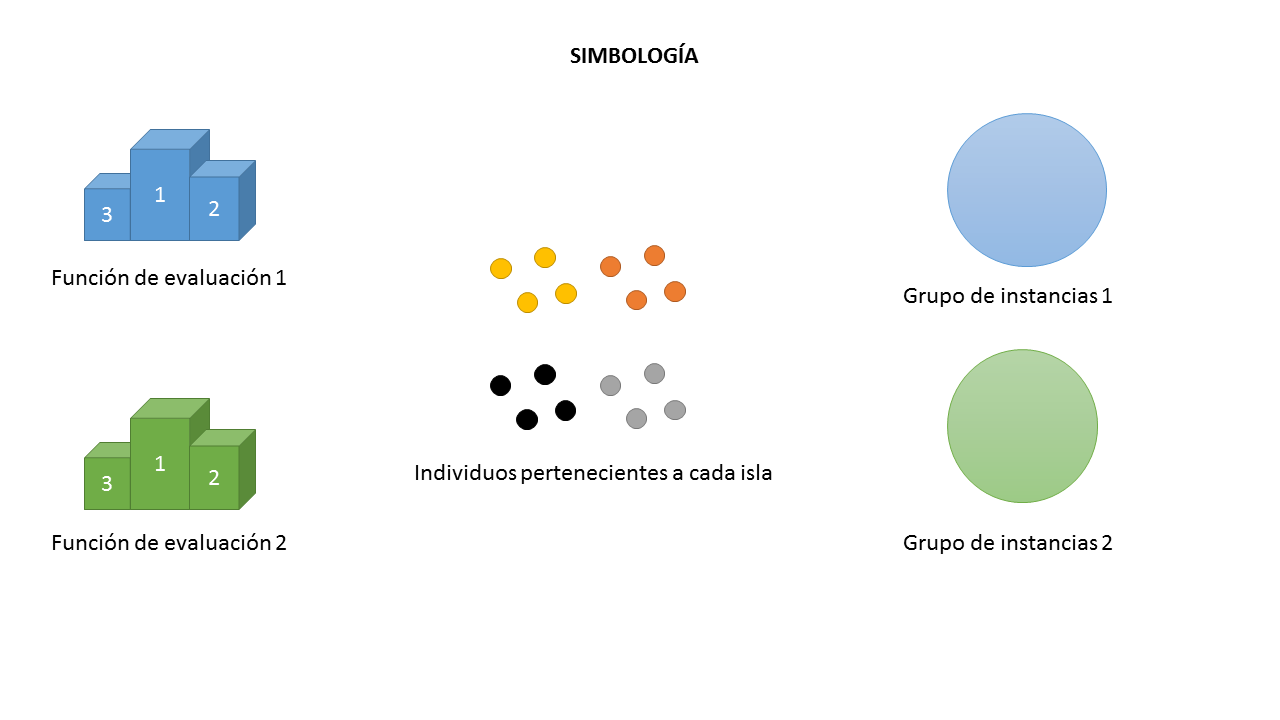
\includegraphics[width=14cm]{images/cap3/simbologia.png}
    \captionof{figure}{Simbología para el método de las islas (Elaboración propia, 2015)}\label{fig:simbologia}
\end{figure}

\begin{figure}[H]
    \centering
    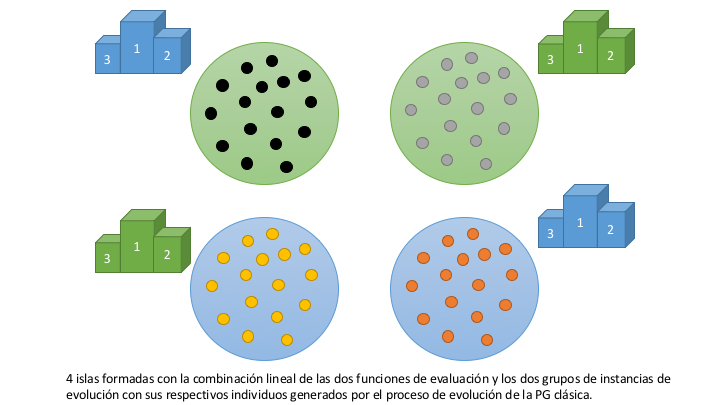
\includegraphics[width=14cm]{images/cap3/estructura.png}
    \captionof{figure}{Estructura de las islas (Elaboración propia, 2015)}\label{fig:estructura}
\end{figure}


El proceso de selección de los individuos que serán enviados a las otras islas se realiza mediante el método de torneo. En la Figura \ref{fig:seleccion} se muestra de forma gráfica la selección, con el fin de obtener los mejores individuos para ser enviados al resto de las islas.

\begin{figure}[H]
    \centering
    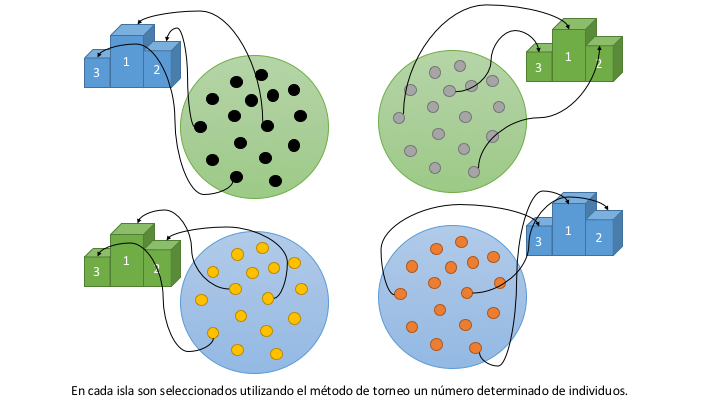
\includegraphics[width=14cm]{images/cap3/seleccion.png}
    \captionof{figure}{Selección de los mejores individuos por isla (Elaboración propia, 2015)}\label{fig:seleccion}
\end{figure}

Posteriormente, los individuos seleccionados son enviados a las demás islas. En la Figura \ref{fig:envio1} se muestra el proceso que ocurre desde una isla, mientras que en la Figura \ref{fig:envio_todos} se puede ver el proceso de intercambio de individuos de forma completa, donde cada una de las islas envía una copia de los individuos seleccionados anteriormente a cada una de las otras islas.

\begin{figure}[H]
    \centering
    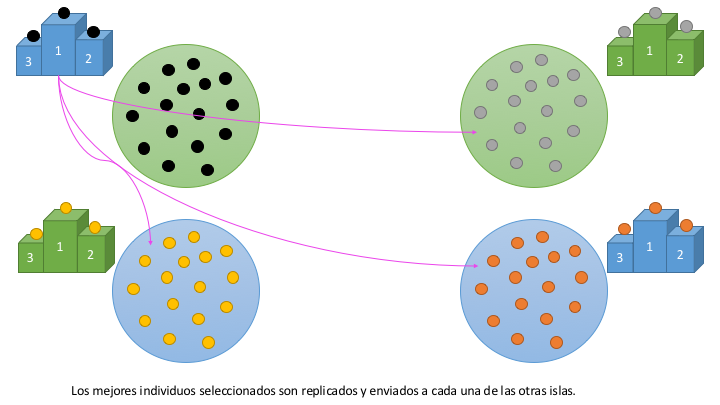
\includegraphics[width=14cm]{images/cap3/envio1.png}
    \captionof{figure}{Isla compartiendo sus mejores individuos a las demás (Elaboración propia, 2015)}\label{fig:envio1}
\end{figure}

\begin{figure}[H]
    \centering
    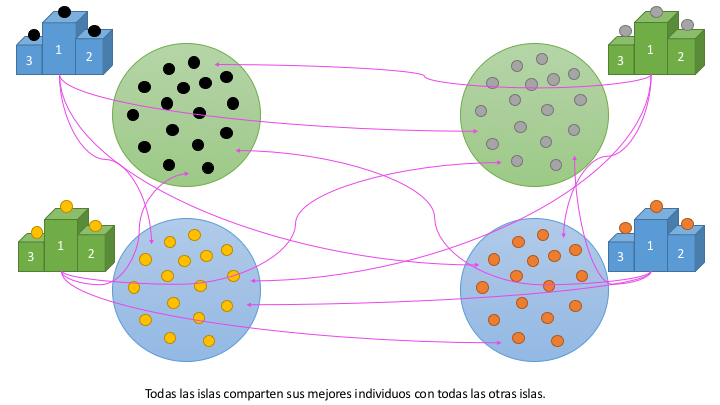
\includegraphics[width=14cm]{images/cap3/envio_todos.png}
    \captionof{figure}{Proceso de envío de mejores individuos entre islas (Elaboración propia, 2015)}\label{fig:envio_todos}
\end{figure}

De forma preparatoria para recibir a los inmigrantes que son enviados por las otras islas, cada una de las islas realiza un torneo inverso, que corresponde a un proceso de selección de los peores individuos para ser eliminados, como se muestra en la Figura \ref{fig:eliminados}.

\begin{figure}[H]
    \centering
    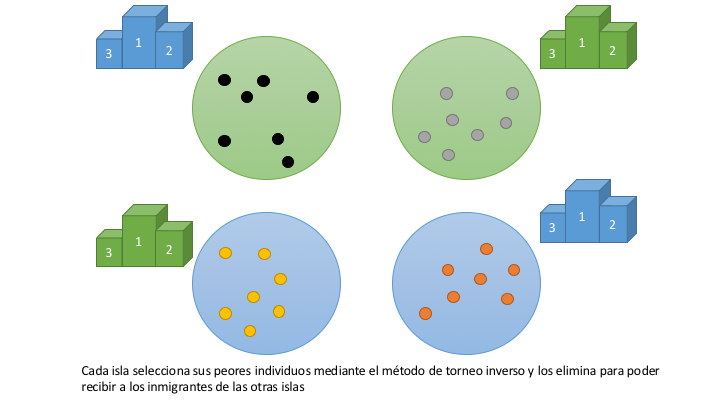
\includegraphics[width=14cm]{images/cap3/eliminados.png}
    \captionof{figure}{Islas luego de eliminar sus peores individuos (Elaboración propia, 2015)}\label{fig:eliminados}
\end{figure}

Finalmente, los inmigrantes pasan a ser parte de la nueva población de cada una de las islas a las que fueron enviados y se procede a continuar con las generaciones del proceso evolutivo de la PG tradicional de cada una de las islas de forma individual, hasta que la condición de compartir individuos sea nuevamente activada. En la Figura \ref{fig:final_islas} se puede ver el resultado luego de recibir cada uno de los individuos de las demás islas.

\begin{figure}[H]
    \centering
    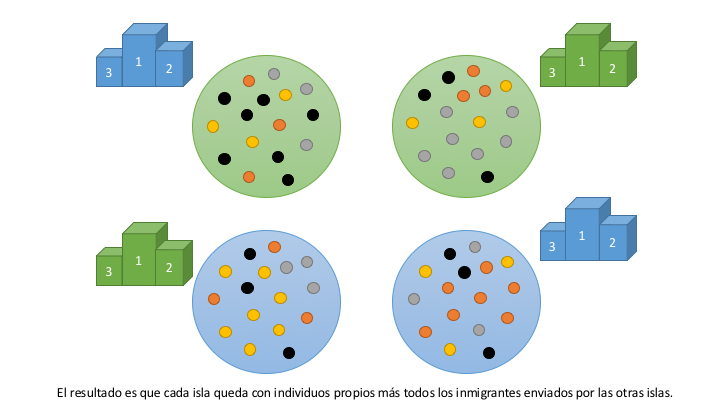
\includegraphics[width=14cm]{images/cap3/final_islas.png}
    \captionof{figure}{Islas luego de realizar la migración de individuos (Elaboración propia, 2015)}\label{fig:final_islas}
\end{figure}

Este proceso evolutivo utilizando la co-evolución con el método de islas puede ser representado con el siguiente diagrama (Figura \ref{fig:pg_islas}). En este diagrama es posible apreciar de forma resumida el proceso descrito anteriormente.

\subsection{El proceso de evaluación}
De igual forma que en el experimento sin co-evolución, este proceso sirve para medir la calidad de los individuos y esta evaluación del desempeño se realiza a través de su ERP. La diferencia con la evaluación del método de PG tradicional es que en este experimento son evaluados los mejores individuos de cada isla mediante su ERP por cada ejecución del proceso evolutivo y no solo el mejor de cada ejecución del proceso evolutivo.

\begin{figure}[H]
    \centering
    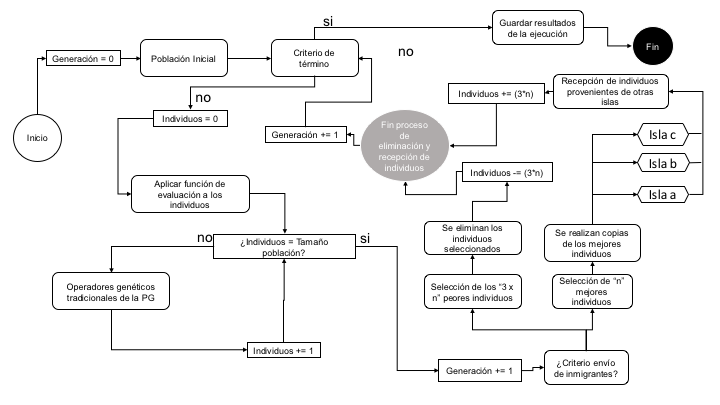
\includegraphics[width=16cm]{images/cap3/pg_islas.png}
    \captionof{figure}{Diagrama de la PG con co-evolución utilizando método de islas (Elaboración propia, 2015)}\label{fig:pg_islas}
\end{figure}

\section{Comparación de experimentos}
Con el objetivo de confirmar o refutar la hipótesis sobre la comparación de los métodos propuestos, se realiza una comparación de los resultados de los experimentos. Estos resultados son sometidos a distintos \textit{test ad-hoc} para comparar cuál de los algoritmos obtenidos mediante el proceso de GAA a través de los experimentos con co-evolución y sin co-evolución es mejor, o si no existe alguna diferencia considerable. Los  \textit{test} a utilizar son los propuestos por \citep{derrac_2011}. Éstos permiten realizar la comparación de los resultados para analizar si existe diferencia o no entre los resultados obtenidos. En la Tabla \ref{tab:comp_exp} se puede apreciar la comparación de los métodos descritos en \ref{cap:experimento_tradicional} y \ref{cap:experimento_islas}. Los valores que no se encuentran especificados son determinados en la sección de parámetros correspondientes a cada problema.


\begin{table}[H]
    \centering
\caption{Comparación entre experimentos (Elaboración propia, 2015)}
\label{tab:comp_exp}
\small
\rowcolors{2}{gray!25}{white}
\begin{tabular}{p{0.35\textwidth}p{0.25\textwidth}p{0.25\textwidth}}\hline
{\textbf{Datos}} & {\textbf{\begin{tabular}[c]{@{}c@{}}Experimento con \\co-evolución\end{tabular}}} & {\textbf{\begin{tabular}[c]{@{}c@{}}Experimento sin \\co-evolución\end{tabular}}} \\ \hline
Estructura de datos                                                     &  \multicolumn{2}{c}{Poseen igual estructura de datos} \\
Funciones                                                               &  \multicolumn{2}{c}{Poseen las mismas funciones} \\
Terminales                                                              &  \multicolumn{2}{c}{Poseen los mismos terminales} \\
Función de evaluación proceso evolutivo                                 & 2 funciones de evaluación: $F1$ y $F2$    &  1 función de evaluación: $\alpha\cdot F1+ \beta\cdot F2$\\
Función de evaluación calidad algoritmos                                &  \multicolumn{2}{c}{Misma función de evaluación mediante el ERP} \\
Casos de adaptación                                                     &  2 grupos de instancias: $G1$ y $G2$      & 1 grupo de instancias $G1 \cup G2$ \\
Casos de evaluación                                                     &  \multicolumn{2}{c}{Poseen el mismo grupo de casos de evaluación} \\
Número de poblaciones                                                   &  4                                     &  1 \\
Tamaño de población                                                     &  $P/4$ por cada población              &  $P$ \\
Número de generaciones                                                  &  \multicolumn{2}{c}{Igual número de generaciones} \\
Probabilidad de cruzamiento                                             &  \multicolumn{2}{c}{Igual porcentaje} \\
Probabilidad de reproducción                                            &  \multicolumn{2}{c}{Igual porcentaje} \\
Probabilidad de mutación                                                &  \multicolumn{2}{c}{Igual porcentaje} \\
Método de generación de población inicial                               &  \multicolumn{2}{c}{\textit{Ramped Half and Half}} \\
Método de selección de individuos                                       &  \multicolumn{2}{c}{Torneo con 4 individuos} \\
Método de selección de nodos                                            &  \multicolumn{2}{c}{\textit{Koza Node Selector}} \\
Probabilidad de selección de nodos                                      &  \multicolumn{2}{c}{90\% terminales y 10\% funciones} \\
Altura máxima de evolución                                              &  \multicolumn{2}{c}{15} \\
Criterio de término                                                     &  \multicolumn{2}{c}{Completar todas las generaciones} \\
Individuos a compartir con otra población                               &  5 (son replicados y compartidos)      & no aplica \\
Poblaciones a las que compartir                                         &  Cada población comparte con todas las demás & no aplica \\
Número de generaciones que la población espera para enviar inmigrantes  &  10                                    & no aplica  \\
Generación en la que se inicia el envío de inmigrantes                  &  1                                     & no aplica  \\
Selección de inmigrantes a enviar                                       &  Torneo con 4 individuos               & no aplica  \\
Selección de individuos a eliminar                                      &  Torneo inverso con 4 individuos & no aplica  \\\hline
\end{tabular}
\end{table}

\section{Consideraciones generales}\label{cap:consideraciones}
Para trabajar con la PG en ambos tipos de experimentos, se tienen en consideración algunos aspectos comunes. Esto debido a que el diseño, construcción, parametrización, calibración y \textit{testing} previo a la ejecución de la PG, es un proceso iterativo en cada experimento, y los efectos de un cambio en el diseño deben implementarse y realizarse \textit{testing}, cada vez, para conocer sus efectos reales. Se realiza a continuación una descripción de las consideraciones.

\subsection{Resultados}
En los experimentos se busca encontrar algoritmos que solucionen los problemas planteados en la Hipótesis, adicionalmente, estos resultados deben dar resultados similares o mejores a los obtenidos en trabajos previos utilizando la PG tradicional para estos problemas.

\subsection{Instancias}
En los experimentos se utilizan instancias disponibles en la \textit{web} para uso investigativo y reconocidas por la comunidad científica asociada al área, las cuales difieren en cantidad para cada problema. La complejidad, división y cantidad a utilizar es especificada en el capítulo correspondiente al diseño del experimento de cada problema.


\subsection{Ejecuciones}
Aunque la PG utiliza generación aleatoria de números, es decir una semilla distinta para cada ejecución, se observa que bastan cinco ejecuciones para probar que los resultados son estadísticamente verdaderos. De acuerdo a \citep{cantu_2003, li_2004} no siempre es necesario realizar múltiples ejecuciones, ya que depende de varios factores como la variabilidad de las funciones, terminales, el problema en sí, entre otros. Es por esto que se realizó un \textit{test} estadístico, utilizando la herramienta STATA (\textit{Data analysis and statistical software}) para comprobar si los datos se encuentran normalizados y posteriormente analizar si existe diferencia entre los resultados entregados por cada una de las ejecuciones realizadas. En la Figura \ref{fig:ejecuciones} se puede ver los resultados de cinco ejecuciones de la PG, donde el mejor individuo de cada una de ellas es evaluado en las 12 instancias con que se realizó la evolución. El \textit{test} de \textit{Shapiro-Wilk} da como resultado que los valores se encuentran normalizados o en algunos casos no existe observación (los resultados son iguales). Posteriormente, se realizó un \textit{test} de ANOVA que con 95\% de confiabilidad intenta probar si los valores poseen alguna diferencia significativa, resultando que no es posible determinar que exista esta diferencia. Por lo mencionado anteriormente, se puede apreciar que no es necesario realizar un gran número de ejecuciones para obtener mejores resultados, ya que éstos no presentan una diferencia significativa.

\begin{figure}[H]
    \centering
    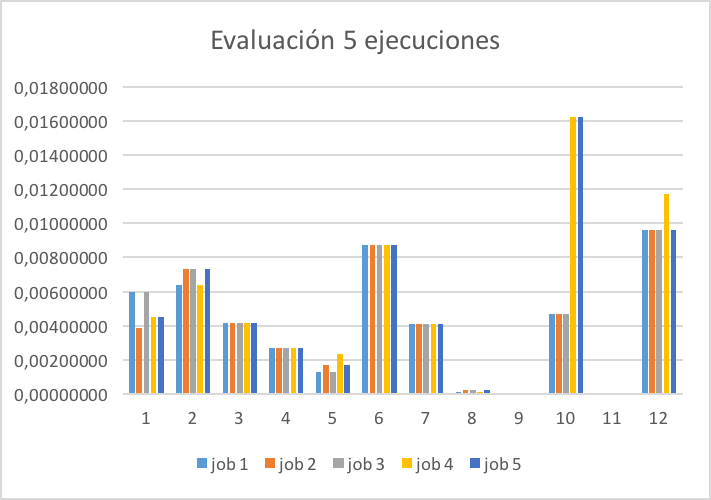
\includegraphics[width=14cm]{images/cap3/ejecuciones.png}
    \captionof{figure}{Evaluación del mejor individuo sobre el conjunto de adaptación (Elaboración propia, 2015)}\label{fig:ejecuciones}
\end{figure}

\subsection{Islas}
En la literatura existen algunos casos donde se utiliza el método de co-evolución mediante islas (véase \ref{cap:rev_coev}). Sin embargo, no existen estudios para especificar el número de individuos que éstas deban compartir. Por otra parte, la calibración óptima de parámetros es otro problema de alta complejidad \citep{karafotias_2014, karafotias_2015} que escapa de los alcances de este trabajo, por lo que se utilizan los valores utilizados en experimentos similares. Estos valores son los siguientes:
\begin{itemize}
  \item Número de individuos a enviar: 5.
  \item Envío a todas las demás islas: Sí.
  \item Número de generaciones que la población espera para enviar inmigrantes: 10.
  \item Generación en la que se inicia el envío de inmigrantes: 1.
\end{itemize}
